% ********************************** Preamble **********************************
% Preamble: Contains packages and user-defined commands and settings

%%-----------------------------------------------------------------------------
%% USE THEME
%%-----------------------------------------------------------------------------
\usetheme{BluePhD}
% \usetheme{PaloAlto} 
% \usetheme{Singapore}
% \usetheme{Szeged}
% \usetheme{CambridgeUS}
% \usetheme{Montpellier}
% \usetheme{Pittsburgh} <---
% \usetheme{Warsaw}
% \usetheme{Rochester}
% \usetheme{Marburg}
% \usetheme{Malmoe}
% \usetheme{Madrid}
% \usetheme{Luebeck}
% \usetheme{Ilmenau}
% \usetheme{Hannover} <---
% \usetheme{Goettingen}
% \usetheme{Dresden}
% \usetheme{boxes}
% \usetheme{Boadilla}
% \usetheme{Berlin}
% \usetheme{Berkeley}
% \usetheme{AnnArbor}

\usepackage{lmodern}
\usepackage[scale=2]{ccicons}

%%-----------------------------------------------------------------------------
% %  double slides left presentation // right notes NOT WORK WELL!!!
%%-----------------------------------------------------------------------------
% \usepackage{pgfpages}
% \setbeameroption{show notes on second screen=right}

%%-----------------------------------------------------------------------------
%%  margins
%%-----------------------------------------------------------------------------
\setbeamersize{text margin left=0.4cm}  % <- like this
\setbeamersize{text margin right=0.4cm} % <- like this

%%-----------------------------------------------------------------------------
%% Set background for theme
%%-----------------------------------------------------------------------------
\setwatermark{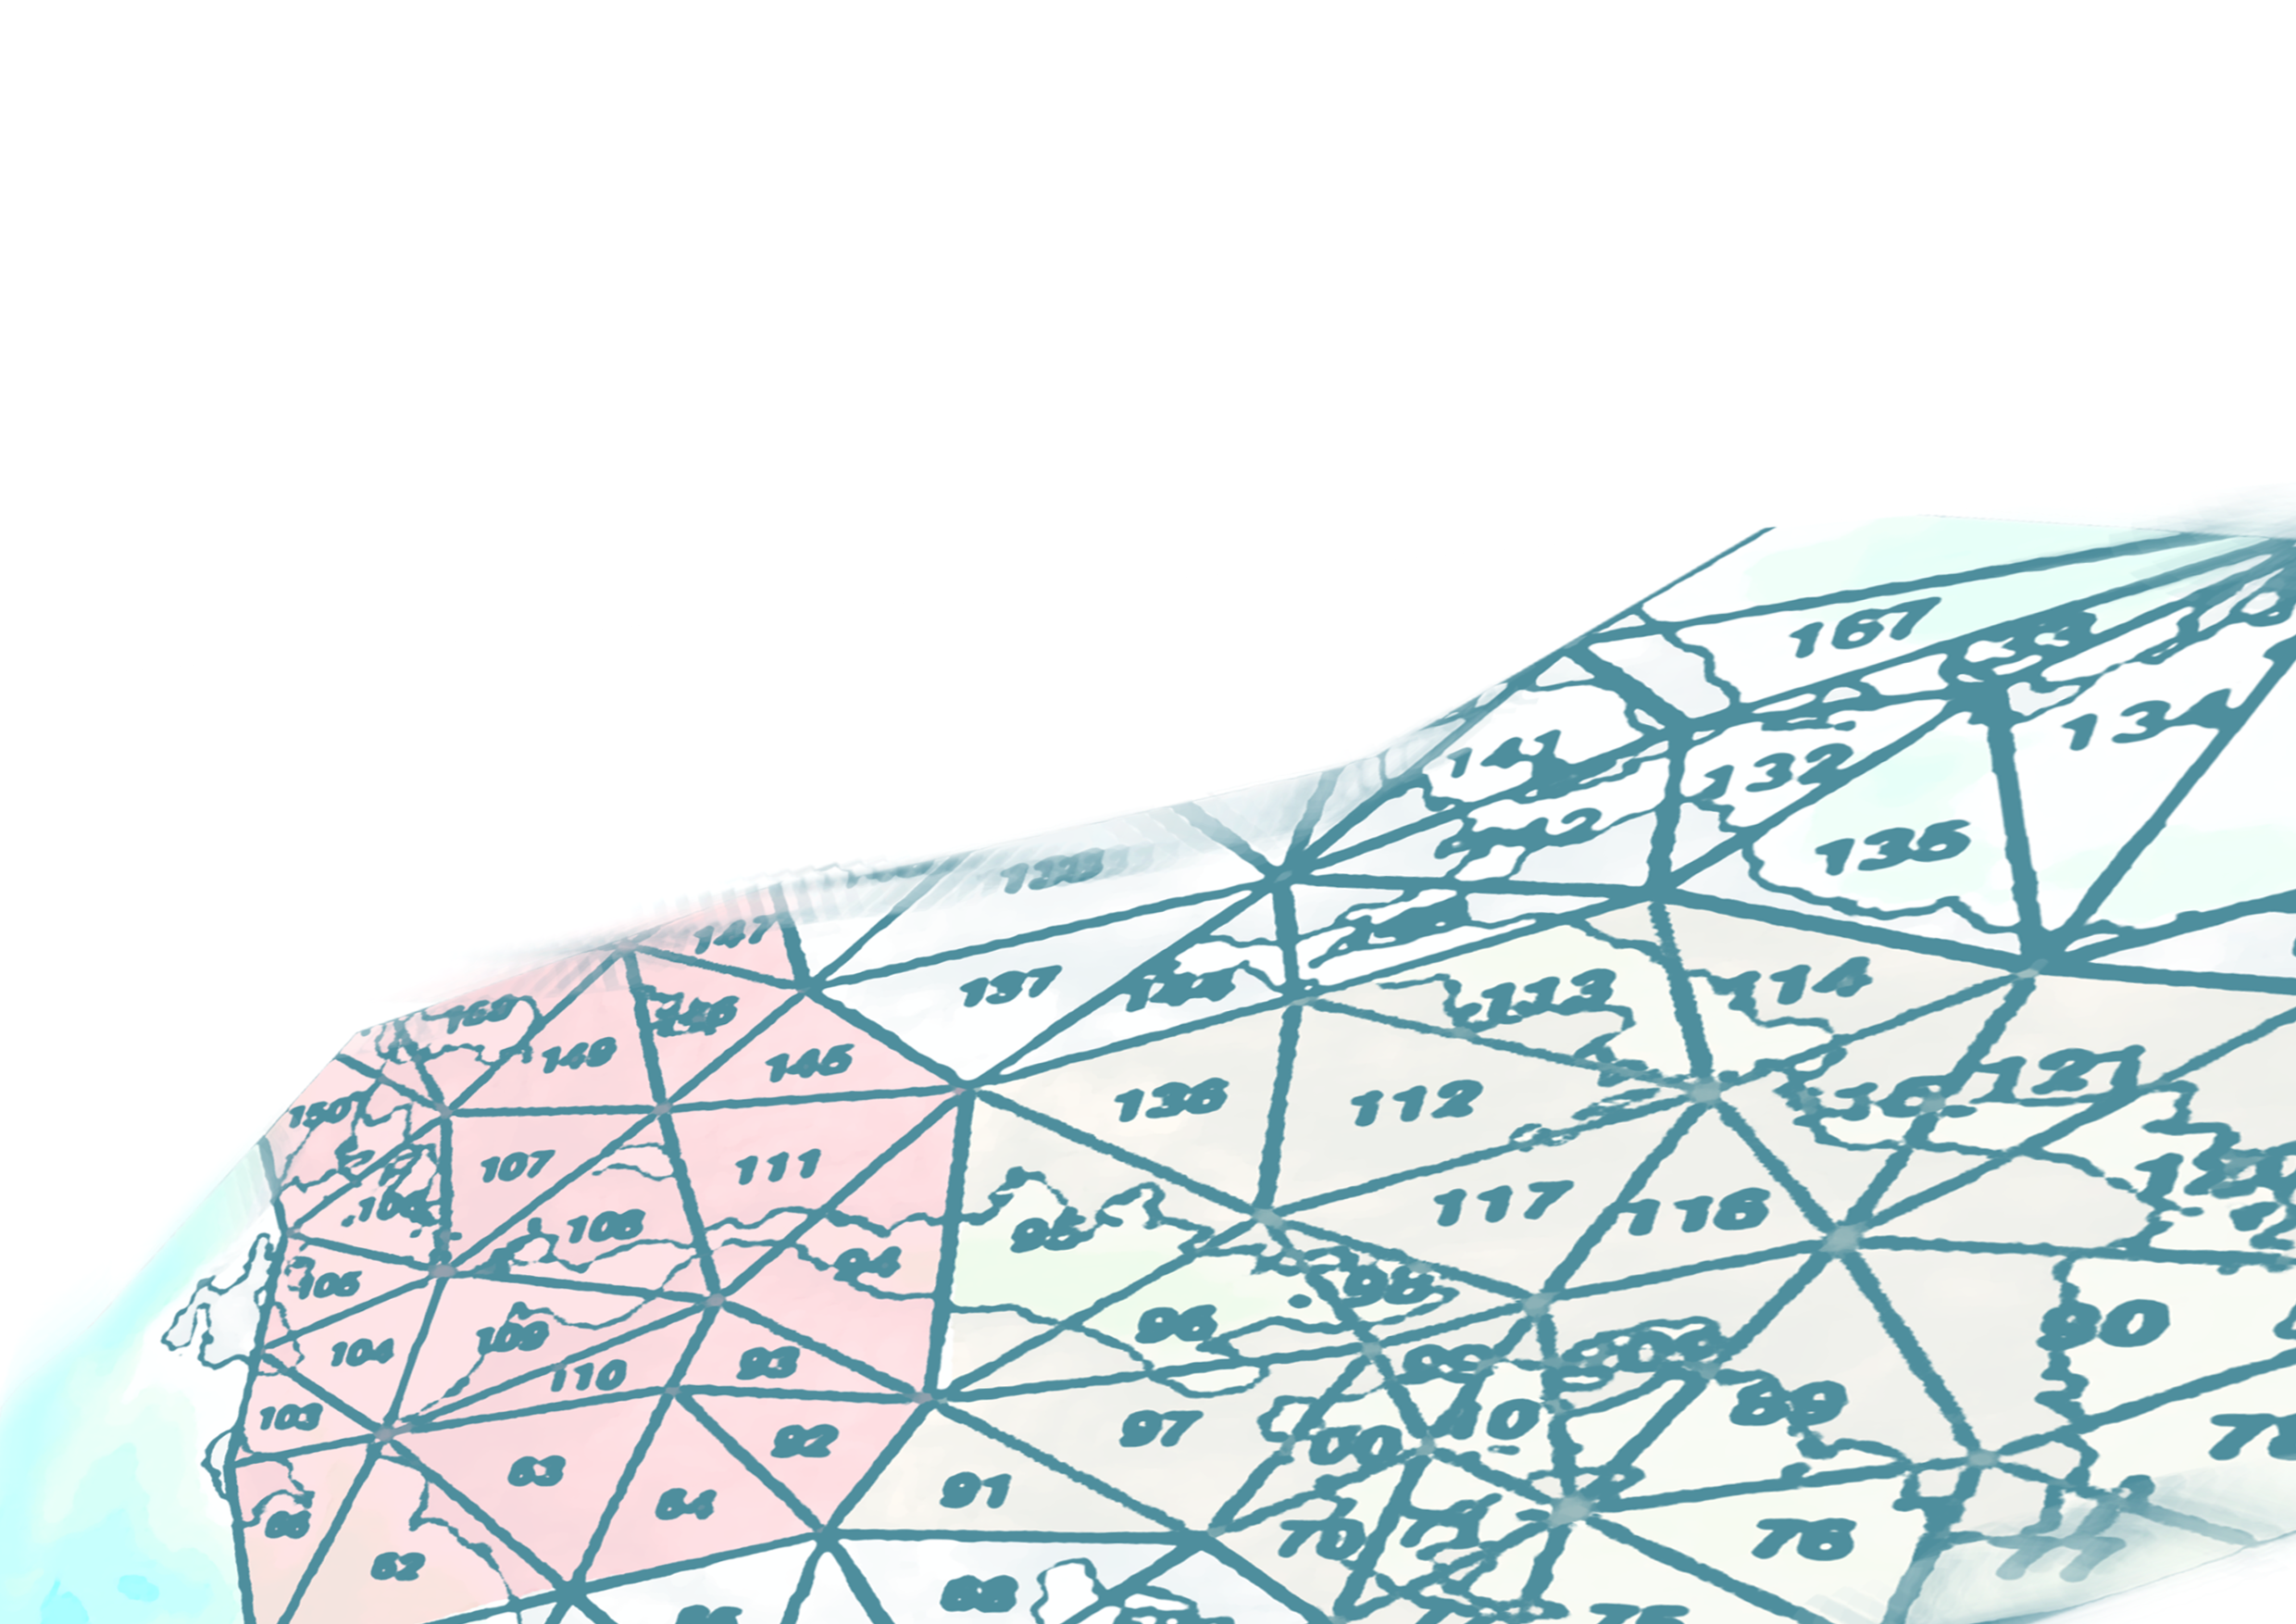
\includegraphics[height=8cm,draft=false]{Figs/backgr01.png}}

%%-----------------------------------------------------------------------------
%% Languages
%%-----------------------------------------------------------------------------
% \usepackage[english, greek]{babel}
\usepackage{xgreek}
\usepackage[Greek,Latin]{ucharclasses}
\setTransitionsForGreek{\setlanguage{greek}}{\setlanguage{english}}
% \usepackage{xunicode}
% \usepackage{xltxtra}
% \usepackage[monogreek]{xgreek}
% \usepackage{tabu}

%%-----------------------------------------------------------------------------
%% Tables
%%-----------------------------------------------------------------------------
\usepackage{booktabs,tabularx}
\usepackage{tabu}
\usepackage{multirow}

%%-----------------------------------------------------------------------------
%% Fonts
%%-----------------------------------------------------------------------------
\usepackage{fontspec}

% Add `customfont' in the document class option to use this section
\ifdefineCustomFont
  \usefonttheme{professionalfonts} % using non standard fonts for beamer
  \usefonttheme{serif} % default family is serif
  \setmainfont[Mapping=tex-text]{GFS Didot}
%  \setmainfont[Mapping=tex-text]{GFS Bodoni}
%  \setmainfont[Mapping=tex-text]{GFS Olga} % ότι να ναι αυτή!!πλάγια NOT support English
%  \setmainfont[Mapping=tex-text]{GFS Neohellenic}
%  \setmainfont[Mapping=tex-text]{GFS Artemisia}
%  \setmainfont[Mapping=tex-text]{GFS Elpis} %low resolution printing
%  \setmainfont[Mapping=tex-text]{Linux Libertine T}
%  \setmainfont[Mapping=tex-text]{Linux Libertine O}

%  % For use with XeLaTeX
%    \setmainfont[
%      Path              = /usr/share/texlive/texmf-dist/fonts/opentype/public/libertine/, %./libertine/opentype/,
%      Extension         = .otf,
%      UprightFont = LinLibertine_R,
%      BoldFont = LinLibertine_RZ, % Linux Libertine O Regular Semibold
%      ItalicFont = LinLibertine_RI,
%      BoldItalicFont = LinLibertine_RZI, % Linux Libertine O Regular Semibold Italic
%    ]
%    {LGR}
%  %  % load font from system font
%     \newfontfamily\libertinesystemfont{Linux Libertine O}

\else
\setsansfont{Arial}

\fi % custom font class


%%-----------------------------------------------------------------------------
% REQUIRED PACKAGES
%-----------------------------------------------------------------------------
\usepackage{graphicx}  % Required for including images
\usepackage{fancybox}
\usepackage{xcolor}
%% for tikz
% \usepackage{dtklogos}
%\usepackage{tikz}
\usetikzlibrary{mindmap,shadows}
\usepackage{smartdiagram}

% restart numbering footnotes per page
\usepackage{perpage}
\MakePerPage{footnote}
% % Sychronize footnotes on columns minipages
\renewcommand\thempfootnote{\arabic{mpfootnote}}

% use nice itemlists ..
%\usepackage{enumitem, color, amssymb}
\usepackage{url}
% \hypersetup{colorlinks,linkcolor=,urlcolor=links}
\hypersetup{colorlinks=true,allcolors=blue}

% use metalogo to print xelatex!
\usepackage{metalogo}

% % tcolorbox custom block, problem with caption package, cant solve it yet!
% \usepackage[most]{tcolorbox}

%%-----------------------------------------------------------------------------
%% Adgust figures
%%-----------------------------------------------------------------------------
\usepackage{adjustbox} % for \adjincludegraphics
% {\shadowbox{\color{black!35}\includegraphics[height=4cm]{img/iono.eps}}

%%-----------------------------------------------------------------------------
%% Print Arrows
%%-----------------------------------------------------------------------------
\usepackage{marvosym} % \MVRIGHTarrow
\usepackage{stmaryrd} % \shortrightarrow $\Rightarrow$
\usepackage{textcomp} % \textrightarrow

%%-----------------------------------------------------------------------------
%% Math symbols
%%-----------------------------------------------------------------------------
\usepackage{amssymb} 
\usepackage{amsmath}

% \usepackage{soul}
% \definecolor{lightblue}{rgb}{.90,.95,1}
% \sethlcolor{lightblue}
% \renewcommand<>{\hl}[1]{\only#2{\beameroriginal{\hl}}{#1}}
% -----------------------------------------------------------------------------
% CAPTIONS
%-----------------------------------------------------------------------------
\usepackage{caption}
\usepackage{subcaption}
\captionsetup[figure]{font=footnotesize,labelfont=footnotesize,skip=0pt,belowskip=0pt}
\setbeamertemplate{caption}[numbered]

\setbeamerfont{caption}{size=\scriptsize}

% -----------------------------------------------------------------------------
% Four Quad
%-----------------------------------------------------------------------------
\newcommand\FourQuad[4]{
    \begin{minipage}[b][.45\textheight][t]{.50\textwidth}\centering#1\end{minipage}\hfill%
    \begin{minipage}[b][.45\textheight][t]{.50\textwidth}\centering#2\end{minipage}\\[0.1cm]
    \begin{minipage}[b][.45\textheight][t]{.50\textwidth}\centering#3\end{minipage}\hfill
    \begin{minipage}[b][.45\textheight][t]{.50\textwidth}\centering#4\end{minipage}%
}

% -----------------------------------------------------------------------------
% Custom symbols for itemize
%-----------------------------------------------------------------------------

\newenvironment{proenv}{\only{\setbeamercolor{local structure}{fg=green}}}{}
\newenvironment{conenv}{\only{\setbeamercolor{local structure}{fg=red}}}{}
 \usepackage{fontawesome}

% -----------------------------------------------------------------------------
% Rotate text
%-----------------------------------------------------------------------------
\usepackage{rotating}
%\begin{turn}{45} 
% ...
% \end{turn}


% -----------------------------------------------------------------------------
% BIBLATEX
%-----------------------------------------------------------------------------
\usepackage{hyperref}
\usepackage[backend=biber,
            style=authoryear,
            maxbibnames=9,
            maxcitenames=1,
            citestyle=authoryear,
            hyperref=true,
            backref=true,
            sorting=nty,
            natbib=true]{biblatex}

% Hypper linc for all citations use \parencite & \textcite
\ExecuteBibliographyOptions{maxcitenames=1}

\DeclareFieldFormat{citehyperref}{%
  \DeclareFieldAlias{bibhyperref}{noformat}% Avoid nested links
  \bibhyperref{#1}}

\DeclareFieldFormat{textcitehyperref}{%
  \DeclareFieldAlias{bibhyperref}{noformat}% Avoid nested links
  \bibhyperref{%
    #1%
    \ifbool{cbx:parens}
      {\bibcloseparen\global\boolfalse{cbx:parens}}
      {}}}

\savebibmacro{cite}
\savebibmacro{textcite}

\renewbibmacro*{cite}{%
  \printtext[citehyperref]{%
    \restorebibmacro{cite}%
    \usebibmacro{cite}}}

\renewbibmacro*{textcite}{%
  \ifboolexpr{
    ( not test {\iffieldundef{prenote}} and
      test {\ifnumequal{\value{citecount}}{1}} )
    or
    ( not test {\iffieldundef{postnote}} and
      test {\ifnumequal{\value{citecount}}{\value{citetotal}}} )
  }
    {\DeclareFieldAlias{textcitehyperref}{noformat}}
    {}%
  \printtext[textcitehyperref]{%
    \restorebibmacro{textcite}%
    \usebibmacro{textcite}}}



\bibliography{References/triangleref.bib}
\newcounter{bibitmctr}
\newcommand{\brf}{%
  \stepcounter{bibitmctr}%
  \ifnum\value{bibitmctr}=7%
    \setcounter{bibitmctr}{0}
    \framebreak
  \fi
}

\renewbibmacro*{finentry}{\finentry\brf}

% % cahnge fontsize of bibliography for biblatex
\renewcommand*{\bibfont}{\tiny}


% -----------------------------------------------------------------------------
% Insert frame after new section
%-----------------------------------------------------------------------------
% comment next lines if you don't like to use this
\AtBeginSection[]{
  \begin{frame}[b]
%   \vfill
  \vspace{\fill}
  \centering
  \begin{beamercolorbox}[sep=8pt,center,shadow=true,rounded=true]{title}
    \usebeamerfont{title}\Large{\insertsectionhead}%
  \end{beamercolorbox}
  \vskip-2cm
  \begin{flushleft}
    {\color{red!20}\rule{0.7\textwidth}{1pt}}\par
    {\color{red!40}\rule{0.5\textwidth}{1pt}}\par
    {\color{red!60}\rule{0.3\textwidth}{1pt}}\par
    {\color{red!70}\rule{0.16\textwidth}{1pt}}\par
    {\color{red!80}\rule{0.08\textwidth}{1pt}}\par
    {\color{red!90}\rule{0.04\textwidth}{1pt}}\par
  \end{flushleft}
  \vspace{.5cm}
%   \vfill
  \end{frame}
}

% -----------------------------------------------------------------------------
% Configure Draft mode
%-----------------------------------------------------------------------------
% *********************** Configure Draft Mode **********************************
\ifsetDraft
  \usepackage[printwatermark]{xwatermark}
  % Bottom
  \newwatermark*[pages=2-,color=red!60,textalign=center,angle=0,scale=.37,xpos=-.2cm,ypos=-.437\paperheight]{\makebox[.9\textwidth]{{\drafttext}\space-\space{\draftVersion}\space{\timestamp}}}
  %Flush right
%  \newwatermark*[pages=2-,color=red!60,textalign=center,angle=90,scale=.35,xpos=.45\paperwidth, ypos=-.7cm]{\makebox[.9\textwidth]{{\drafttext}\space-\space{\draftVersion}\space{\timestamp}}}
  
\fi 

% Uncomment to disable figures in `draft' mode
% \setkeys{Gin}{draft=true}  % set draft to false to enable figures in `draft'

% These options are active only during the draft mode
% Default text is "Draft"
\SetDraftText{DRAFT}

% Draft Version - default is v1.0
\SetDraftVersion{v1.0}

% ******************************** Todo Notes **********************************
%% Uncomment the following lines to have todonotes. % Not working yet!
%
%\ifsetDraft
%   \usepackage[colorinlistoftodos,prependcaption,textsize=small]{todonotes}
%   \setlength{\marginparwidth}{2.2cm}
%   %\usepackage[colorinlistoftodos]{todonotes}
%   \newcommand{\mynote}[1]{\todo[author=mitsos,size=\small,inline,color=red!40]{#1}}
%   %\newcommand{\unsure}[1]{\todo[author=mitsos,size=\small,color=red!60]{#1}}
%   %\newcommand{\change}[2][1=]{\todo[author=mitsos,size=\small,linecolor=blue,backgroundcolor=blue!35,bordercolor=blue]{#1}}
% % 	\newcommand{\info}[2][1=]{\todo[linecolor=OliveGreen,backgroundcolor=OliveGreen!25,bordercolor=OliveGreen,#1]{#2}}
% % 	\newcommand{\improvement}[2][1=]{\todo[linecolor=Plum,backgroundcolor=Plum!25,bordercolor=Plum,#1]{#2}}
%\else
%    \newcommand{\todo}[1]{}
% 	\newcommand{\mynote}[1]{}
%% 	%\newcommand{\unsure}[1]{}
%% 	%\newcommand{\change}[1]{}
%% 	%\newcommand{\info}[2][1=]{}
%% 	%\newcommand{\improvement}[2][1=]{}
%% 	%\newcommand{\listoftodos}{}
%\fi
%%
%% Example todo: \mynote{Hey! I have a note}
